Para tener claro el orden de resolución y aparición de los puzzles, se ha realizado una gráfica jerarquizada. El primer puzzle de \nombrejuego sería el tutorial, el más arriba de la jerarquía. El último sería el examen de la Junta Directiva.

\begin{figure}[H] 
	     \begin{center}
	         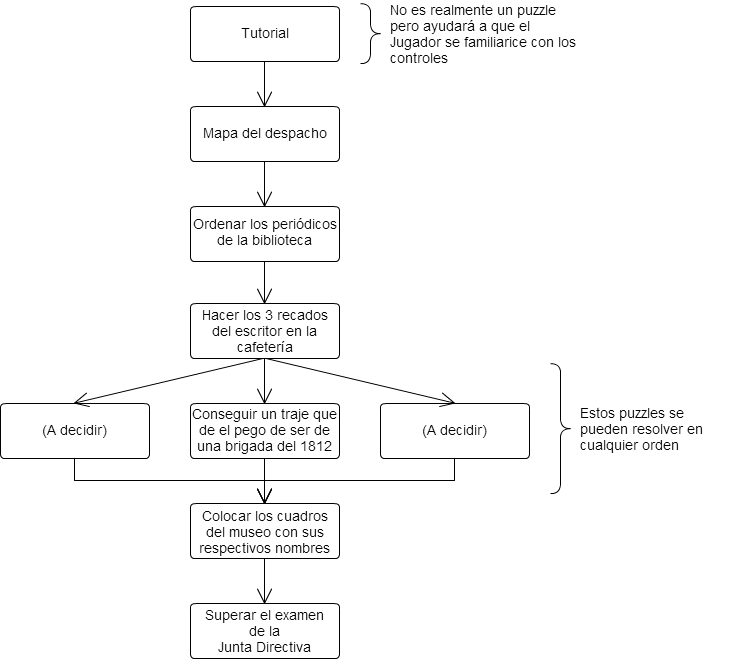
\includegraphics[scale=0.5]{estructura-puzzles.png}
	     \end{center}
	     \caption{Orden de aparición y resolución de los puzzles de \nombrejuego}
	     \label{fig:estructura-puzzles}
	\end{figure}